% !TEX root = main.tex
\begin{figure*}[h!]
	\center
	\includegraphics[width=\linewidth]{DPPC_Only.pdf}
	\caption{nAChR boundary lipids in binary mixtures of DPPC and CHOL. A: Representative frame from a simulated trajectory of a single nAChR embedded in a small membrane, colored by subunit ($\alpha$:green, $\beta$:purple, $\delta$:gray, $\gamma$:cyan) in a 4:1 DPPC (blue):Chol (red) mixture.  B: Extent of demixing ($M_{DPPC,DPPC}$ defined in Eq. \ref{eq:M}) and depletion of saturated lipids from the boundary ($\qsat$ defined in Eq.\ref{eq:Q}) in small binary membranes. In this binary system, cholesterol depletion/enrichment is directly related to the saturated lipid depletion/enrichment: $Q_\mathrm{chol}=-x_{\mathrm{sat}} \qsat/\xch$.  Error bars represent standard error for a blocking average over 50 ns. C: Average normalized density (Eq. \ref{eq:Rt}) of cholesterol for the system in A. Plot shown is identical to Figure \ref{fig:sorting} in ``Chol'' row, ``None'' column, but has been cropped and zoomed around the protein center.\grace{Update previous sentence upon inclusion of new figure}}
	\label{fig:binary}
\end{figure*} 
\subsection {Spontaneous association with cholesterol in binary membranes} \label{binary}

%We previously proposed that cholesterol could be embedded within intersubunit and intrasubunit sites of \nachr\cite{Brannigan_Embedded_2008} or intersubunit sites of the GABA(A) receptor\cite{Brannigan_Embedded_2008}.  It was recently found in \cite{Laverty2017}, to embed within the inter- and intra-subunits of nAChR and other pLGICs. Docking has been used in previous computational research to determine optimal cholesterol binding domains \cite{Hnin_A_2014,Brannigan_Embedded_2008}, but coarse grained systems have shown to be a novel method to simulate non-annular lipid binding without the need to dock lipids within proteins. \liam{Figure \ref{fig:binary} measures an absence of embedded DPPC but an enrichment of cholesterol embedding throughout the protein.}
Lipid sorting was characterized for \nachr s in binary DPPC:CHOL membranes (Figure \ref{fig:binary}A)  using several metrics. 
Non-random lipid mixing (including domain formation) was quantified using the self-association metric $M_{A,A}$ as defined in Equation \ref{eq:M}. %; this quantity reflects degree of self-association of DHA-containing and LA-containing lipids respectively.  %enrichment of lipid species $B$ among the nearest neighbors of lipid species $A$ , with values close to 0 indicating random mixing, and positive and negative values indicating enrichment or depletion of species $B$ around species $A$, respectively. $M_{A,B}>> 0$ indicates substantial demixing and domain formation.  
As expected, in simulated binary membranes containing only DPPC and 0-40\% cholesterol, minimal demixing was observed, with values of $M_{DPPC,DPPC}$ (Fig \ref{fig:binary}B) rising slightly for higher cholesterol concentrations but remaining persistently below 0.05.  %Similar values were observed for $M_{CHOL,CHOL}$.

Depletion of saturated lipids among \nachr~boundary lipids (relative to those expected for a random mixture) was quantified using the metric $\qsat$ defined in equation \ref{eq:Q}. Negative and positive values of $\qsat$ reflect depletion or enrichment of saturated lipids in the \nachr~boundary, respectively. In binary systems containing cholesterol and saturated lipids, depletion of saturated lipids corresponds directly to enrichment of cholesterol: $Q_{chol} = -\qsat x_{sat}/\xch$. %, respectively, while values of $\qsat$ approaching 1 or -1 indicates partitioning within a well-defined $\lo$ or $\ldo$ phase, respectively.

In binary DPPC:CHOL mixtures, $\qsat$ was very slightly negative for $\xch < 20\%$, but decreased steadily for higher concentrations. This trend indicates some depletion of DPPC (and enrichment of cholesterol) among \nachr~ boundary lipids (Figure \ref{fig:binary}B).  Typically, between 10 and 20\% cholesterol has been required in reconstitution mixtures to restore native function  \cite{Fong_Correlation_1986,Dalziel1980,Criado1982}  and a phase transition at about 20\% cholesterol in binary DPPC:CHOL model membranes is indicated by differential scanning calorimetry.\cite{Marsh2010} 

Spontaneous binding of cholesterol to non-annular or ``embedded'' sites, similar to what we previously proposed\cite{Brannigan_Embedded_2008}, was observed in these CG-simulations, and penetration of the TMD bundle by DPPC acyl chains was also observed at lower cholesterol concentrations (Fig \ref{fig:binary}A).  Distribution of density for embedded lipids is further discussed in Section 3.4.  %deep binding of lipids was much more common in the subunit interfaces, particularly $\alpha/\beta$ and $\delta/\alpha$, than in the subunit center (Figure \ref{fig:sorting})\liam{. A}lthough DPPC partitioned extensively to the relatively large cavity in the center of the $\beta$ subunit.  

Annular cholesterol (enrichment of cholesterol at the protein-lipid interface), is visible for the binary systems via a ring of high (red) cholesterol density just around the protein in Figure \ref{fig:binary}C. Enrichment of cholesterol near the protein is highly localized with a ring that is less than 5\AA~wide. This is in general agreement with evidence for annular cholesterol in randomly-mixed binary membranes. \cite{Barrantes2010}

%at low concentrations of cholesterol, \liam{it is} almost entirely within ``embedded'' or non-annular \liam{region of the protein} (Figure \ref{fig:binary}C) as predicted in \cite{Brannigan_Embedded_2008}.
%Intriguingly, all simulations consistently yielded four general regions of differential embedded cholesterol density : a high density region ($\alpha_{\gamma}/\gamma$ interface and center of the $\alpha$ subunit), a low/background density region ($\beta/\alpha_{\gamma}$ interface and center of $\beta$ subunit) on the opposite face of the TMD, and two regions of intermediate density that separated them.  In the absence of nAChR, DPPC/CHOL lipid bilayers are randomly mixed, so this result indicates an intrinsic cholesterol amphipathy.  

%At higher concentrations of cholesterol, cholesterol was also enriched in ``annular'' sites, particularly at the high affinity and low affinity face of the TMD.  This enrichment actually extended many lipidation shells off the high affinity face, indicating nAChR was not just sorting lipids, but even inducing organization of the membrane. Enrichment far from the TMD is expected to be particularly sensitive to finite size effects, although there is no clear reason for why these effects would consistently have a dependence on protein orientation.  
% , and two intermediate density regions (1: $\gamma-/\alpha+$ face and subunit center of both subunits and 2: ) and $\delta-/\alpha+$ faces, and nearly background density on the $\alpha-/\beta+$ face.  As a result, the protein overall 


\subsection {Domains formed in PUFA-containing ternary membranes are not affected by introduction of an \nachr } \label{Demix}
	\begin{figure}[h!]
		\center
		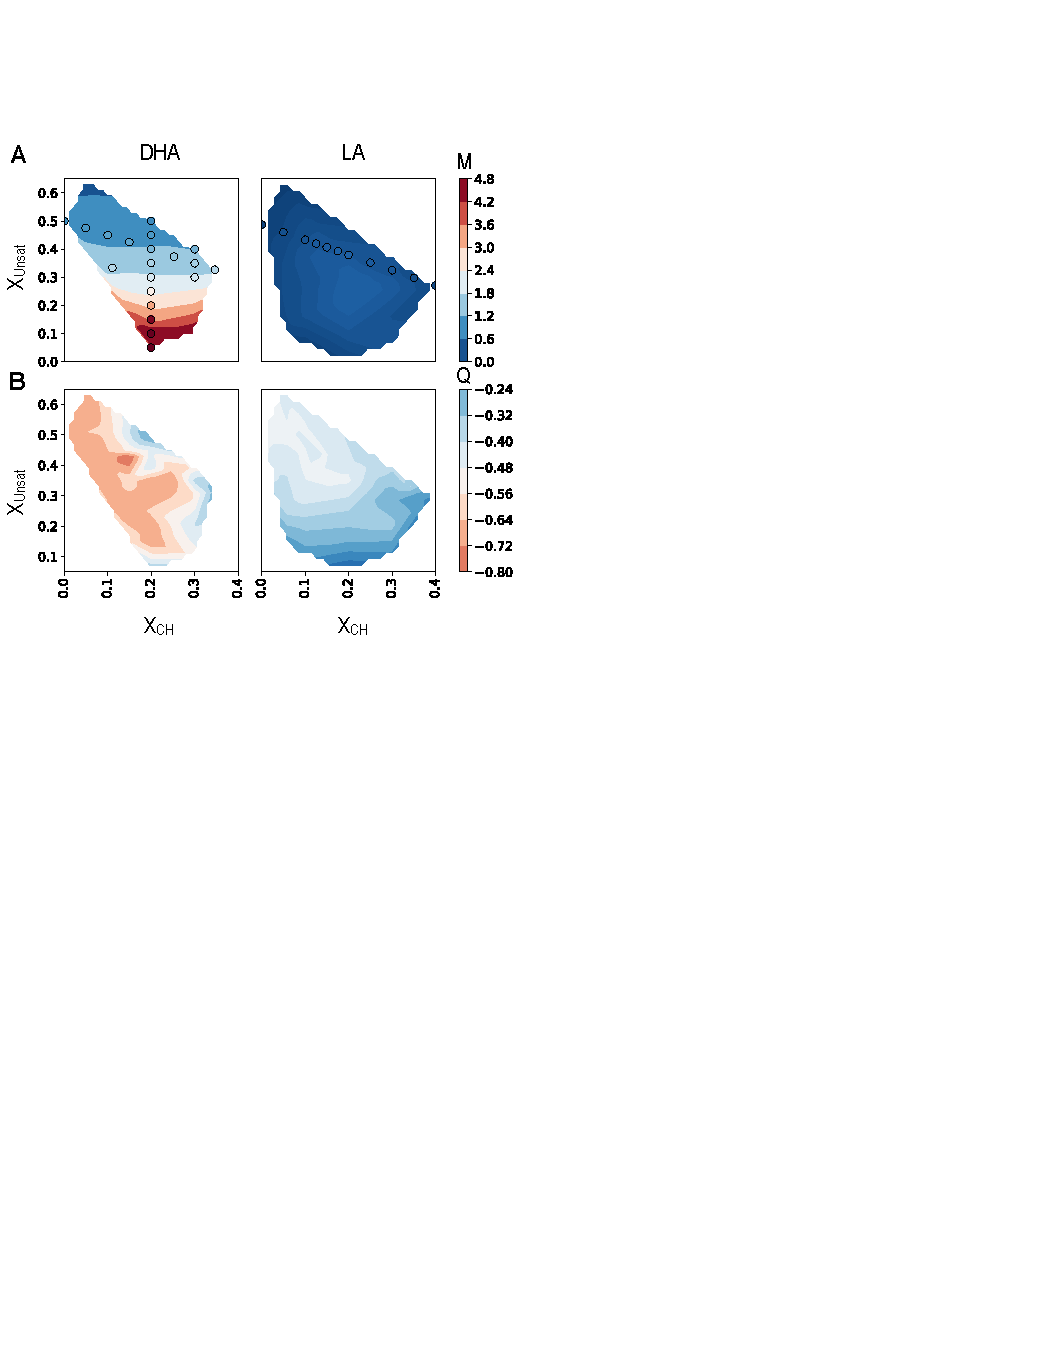
\includegraphics[width=1\linewidth]{Fig2.pdf}
		\caption{Quantitative analysis of bulk membrane mixing and nAChR boundary lipid composition across small membranes containing DPPC, Cholesterol, and either dDHA-PE or dLiPC. Shaded contours were constructed based on 40 individual simulations with DHA and 30 with LA. A: $M_{PUFA, PUFA}$, defined in eq \ref{eq:M}.  Circles represent mixing of systems with the same lipid composition but no \nachr. B: $\qsat$, defined in Eq \ref{eq:Q}.   }
		\label{fig:fig2}
	\end{figure} 
	
	In order to test whether \nachr~affected domain formation in domain-forming membranes, we characterized $M_{{PUFA,PUFA}}$ for systems containing DPPC, Cholesterol, and PE or PC with either n-3 (DHA) or n-6 (LA) acyl chains.   Addition of phospholipids with unsaturated acyl chains to systems containing a saturated lipid and cholesterol is well-established to induce domain formation, and polyunsaturated phospholipids make these domains more well-defined\cite{Levental_Polyunsaturated_2016}. As expected, we observed that addition of PUFAs to DPPC/CHOL bilayers did induce domain formation over a range of compositions, and values for $M_{{PUFA,PUFA}}$ are shown as filled symbols in Figure \ref{fig:fig2} A. 
	
	Introducing a single nAChR to these same systems did not significantly affect domain formation. $M_{DHA,DHA}$ was determined for an isolated \nachr~in ternary mixed membranes with over 40 different combinations of DHA, DPPC, and Cholesterol (Figure \ref{fig:fig2}A, shaded contours). Its effect on membrane organization is represented by the difference in color of the circular symbol and the shaded contour at the same composition.  Introducing a single nAChR into the DHA-containing systems does slightly reduce the amount of DHA required to obtain a given value of $M_{DHA,DHA}$. %, %the difference increased at high DHA concentrations (i.e. $\sim \geq30\%$) and
	%which
	{ This subtle trend} may reflect increased likelihood of DHA-DHA interactions due to nucleation of DHA-containing lipids around the protein (Figure \ref{fig:fig1}). 

	Across ternary mixtures with two long $n-3$ PUFA chains (DHA) and a PE headgroup, maximum values of $M_{DHA,DHA}$ approached 5 (Figure \ref{fig:fig2}A), and were significantly reduced (to less than 0.5) when DHA chains were replaced with linoleic acid (LA) chains. This result is consistent with a previously-observed significant increase in miscibility temperature upon supplementation of plasma membranes with $n-3$ lipids.  \cite{Levental_Polyunsaturated_2016} 
	
	Substantial lipid demixing in DHA-containing mixtures was observed even at low cholesterol concentrations. Over the range we tested, $M_{DHA,DHA}$ was not sensitive to cholesterol concentration $\xch$, as shown by the horizontal contours for DHA in Figure \ref{fig:fig2}A.   
	%	
%	As shown in Figure \ref{fig:fig2}\textbf{a},  $M_{DHA,DHA}$ actually increases as the molar fraction of DHA-PE is reduced from the membrane, implying increased self-association of DHA at reduced concentrations of DHA, with even the lowest concentrations of DHA that we used here seemingly higher than the critical miscibility concentration.  $M_{DHA,DHA}$ is not sensitive to the ratio of cholesterol vs saturated lipid, at least over the compositions simulated.   Relative to systems containing DHA, $M_{LA,LA}$ implies miscibility fo systems containing LA, with small amounts of domain formation sensitive to the CHOL:DPPC ratio; an apparent maximum for $M_{LA,LA}$ occurs near 20\% LA, 20\% Cholesterol, and 60\% DPPC.  
	%This is consistent with previous work, \cite{Inglfsson_Lipid_2014,Risselada_The_2008,Perlmutter_Interleaflet_2011,Veatch_Organization_2002}, indicating domain formation in ternary mixtures to be primarily dependent on differences in acyl chain unsaturation and relatively insensitive to head group.
%The well-defined boundaries between domains that were found in systems containing DHA-PE are also observed in systems containing DHA-PC. Shorter acyl chains and greater saturation did not promote well defined domains as seen using DHA (see Figure \ref{fig:fig1}A). DHA is a relatively long chained n-3 fatty acid making it highly flexible. DHA has been shown to stabilize $\ldo$ domain formation \cite{Levental_Polyunsaturated_2016,Lor2015}.  It may be the case running our simulations for longer time would produce well defined domains for any DLiPC/PE \cite{Risselada_The_2008}.

\subsection{nAChR consistently partitions to the liquid disordered domain} \label{PUFA}
	For more than 100 lipid compositions tested, nAChR always partitioned into a PUFA-rich $\ldo$ phase if such a phase was present. We never observed \nachr~partitioning to an $\lo$ phase. Representative frames from trajectories of domain formation in the presence of \nachr~are shown in Figure \ref{fig:fig1}.  This observation includes all tested concentrations of the ternary mixtures, regardless of whether the zwitterionic headgroup was PC or PE (Figure \ref{fig:SIQ}), or whether DPPC was replaced by dioleoylphosphatidylcholine (DOPC) (di-18:1), Palmitoyloleoylphosphatidylcholine (POPC) (16:0,18:1), or dilauroylphosphatidylcholine (DLPC) (di-14:0), as shown in Figure SI\ref{fig:OL}.   %\liam{This is independent of acyl chain length, but dependent on the level of unsaturation, as seen in .} If PUFAs were included, unsaturated lipids were enriched and saturated lipids depleted from the boundary.}  
	
	% within a randomly mixed ternary membrane, then allowing the membrane to de-mix and nAChR to explore domains, reveals nAChR to partition into the $l_d$ domain if a $l_d$ domain is present. 
		%	Similarly, %\ref{fig:OL}, 
	%partitioning to the disordered domain was qualitatively insensitive to headgroup (PE or PC) for the compositions simulated. 
	%In  heat maps describing the boundary DPPC near nAChR. 
	{These results are quantified for \nachr~embedded in ternary membranes containing DPPC, CHOL, and either DHA-PE or dLiPC\grace{We repeatedly use LA rather than Li, is there a reason?} in Figure \ref{fig:fig2} B, using the metric $\qsat$ defined in equation \ref{eq:Q}.}  %   indicating partitioning within the $\l_{d}$ phase, Q = 0 indicates random partitioning, and Q = 1 indicates enrichment of DPPC lipids, indicating partitioning within the $l_{do}$ phase (Figure \ref{fig:fig2}\textbf{b}).  
	In all systems studied here, $\qsat < 0$, indicating depletion of saturated lipids as boundary lipids, consistent with observed partitioning to the $\ldo$ domain in Figure \ref{fig:fig1}. Furthermore, depletion was much stronger in systems containing DHA ($\qsat^{DHA}<< \qsat^{LA}$), consistent with the more well-defined DHA domains ($M_{DHA,DHA}>> M_{LA,LA}$). %{ for n-3 PUFAs were noticeably more negative than $\qsat$ for n-6 PUFAs}.   %From $\qsat$ alone it is not clear whether this difference reflects a significantly higher affinity of nAChR for $n-3$ DHA than $n-6$ LA or simply the more well-defined $\ldo$ phase formed by DHA compared to LA. 	%The color bar in Figure \ref{fig:fig2}\textbf{b} represents $Q$. 	 
	%We did consistently measure $\qsat<0$ regardless of restraints place on the protein or box size (Figure \ref{fig:fig2}C). % shows harmonic restraints in a membrane $\sim 75x75nm^2$.  
	%fig? was the cth figure in figure one, we replaced it with the large simulation image.
	%Both saturation and acyl chain length dictate domain formation. 
		\begin{figure*}[t]
		\center
		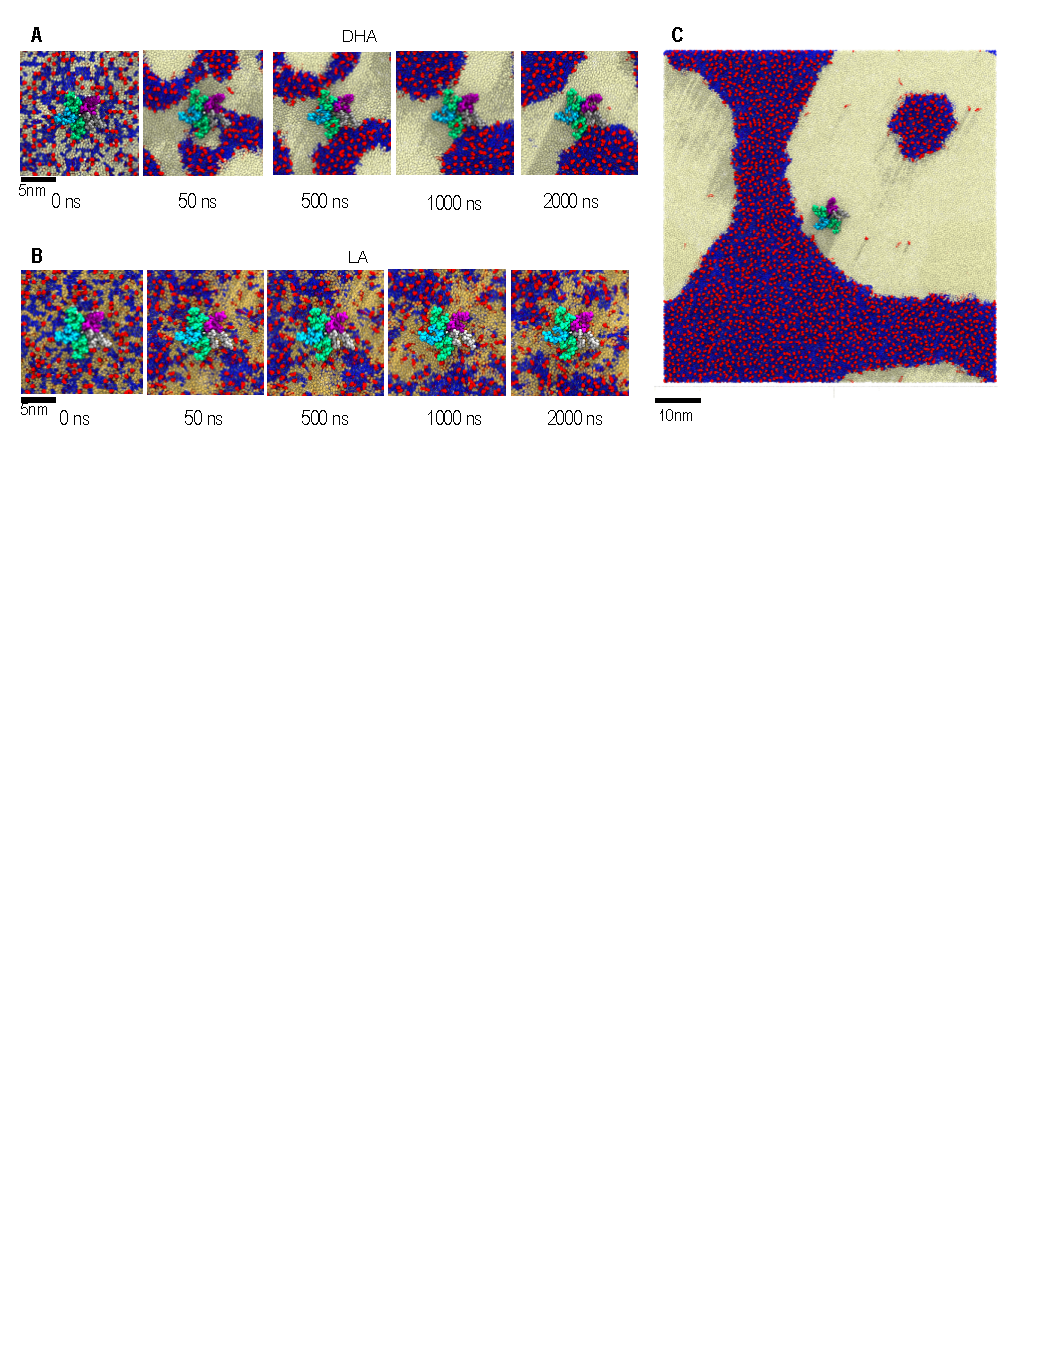
\includegraphics[width=1\linewidth]{Fig1.pdf}
		\caption{ Trajectories of ternary mixtures at ratios of 2:2:1 DPPC:PUFA:Chol. A and B: Trajectories of simulation systems with a single nAChR embedded within small membranes, using lipids containing DHA acyl chains or LA acyl chains. Both simulations were run for 2 $\mu$s. C: Final snapshot of 4 $\mu$s trajectory of a system within a large $\sim$ 75x75 nm$^2$ membrane with the same composition as in A. Subunits are colored: $\alpha$: green, $\beta$: purple, $\delta$: gray, $\gamma$: cyan. Lipids are colored: Chol: red, DPPC: blue, di-DHA-PE: white, DLiPC: tan.} 
		\label{fig:fig1}
	\end{figure*}

	\begin{figure}[!ht]
		\center
		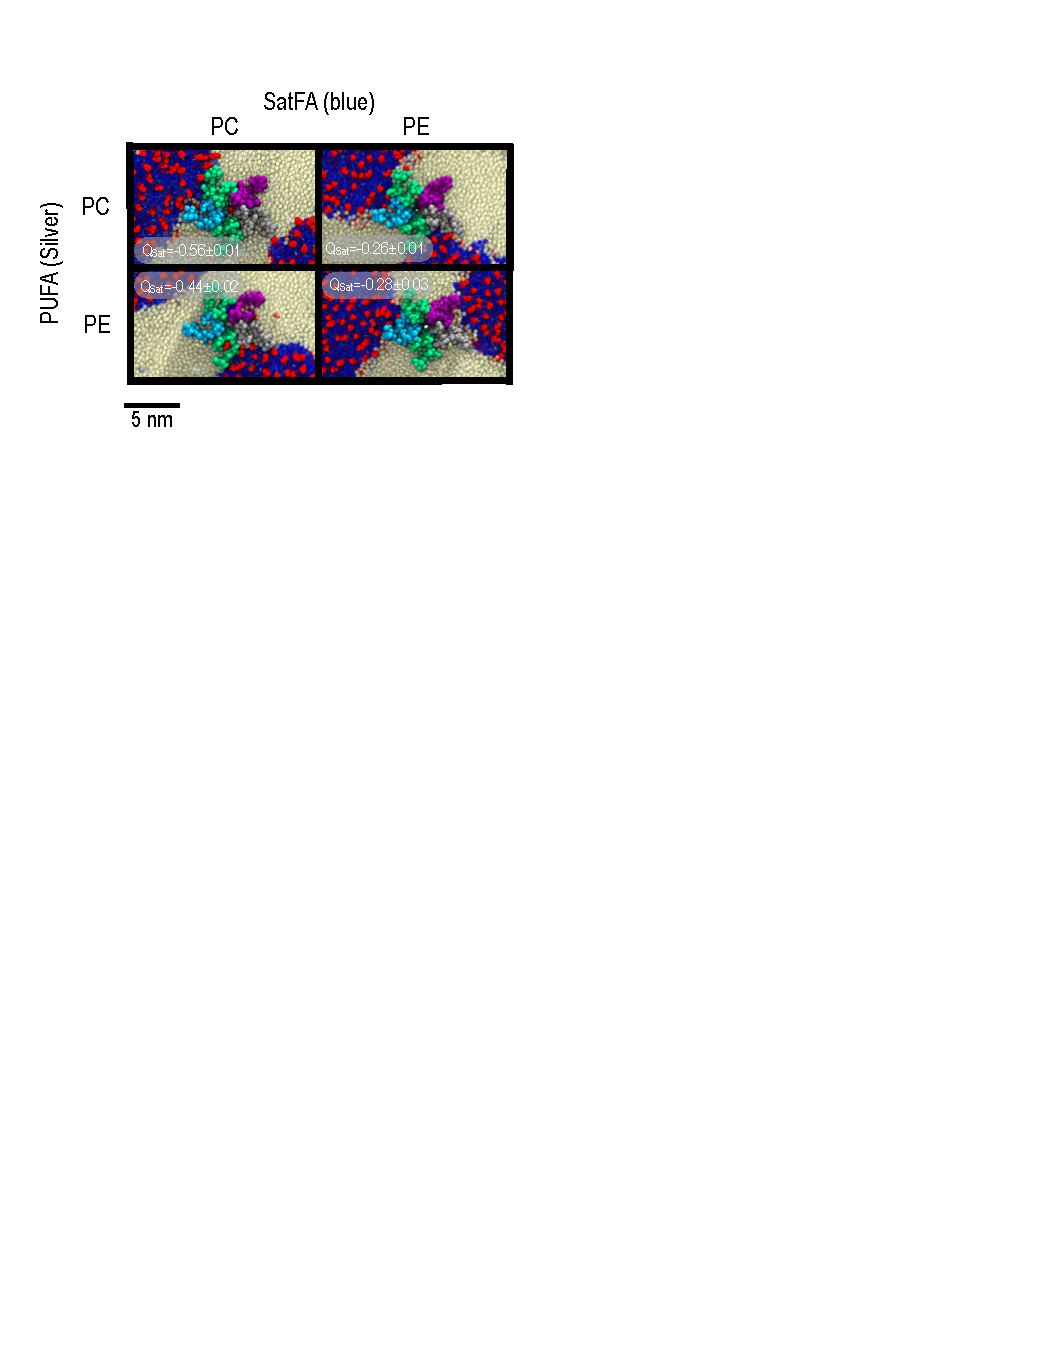
\includegraphics[width=1\linewidth]{SI_Q.pdf}
		\caption{ Comparison of nAChR partitioning based on lipid headgroups (PC and PE). All images represent last frame of 2$\mu$s  simulations of small membranes with composition  2:2:1 Sat:PUFA:Cholesterol.  Rows represent the head-group for the PUFA-containing lipid, while columns represent the head-group of the saturate lipid.   Each image includes $\qsat$ values related to individual systems with errors across averaging 50~ns blocks.}
		\label{fig:SIQ}
	\end{figure}
	%\liam{\cite{Parton2013,Goose2013,Scott2008}, which used multiple proteins assisted in membrane organization,
	%Since 
	%the single \nachr~molecule used within these experiments does not significantly affect membrane organization, which is instead driven by lipid-lipid interactions.} 
	
	The \nachr~annulus is highly enriched in DHA: DHA-PE constitute nearly 100\% of the local lipids even in membranes with very low DHA concentrations. This strong signal could indicate multiple high affinity sites for DHA chains across the transmembrane protein surface. At another extreme, DHA enrichment could be driven by a very slight preference for DHA in a highly non-ideal bulk: since DHA is found in well-defined domains without protein, even one DHA molecule that binds to the protein surface could stabilize the rest of the $\ldo$ domain nearby. Comparing boundary lipid and domain formation trends can help distinguish between these two scenarios.  If boundary lipid enrichment is determined purely by how well-defined domains are (the latter scenario), we would expect similar trends for $M_{DHA,DHA}$ and $Q_{sat}$ in the DHA column of Figure \ref{fig:fig2}.  In contrast,  Figure \ref{fig:fig2} shows that while domain formation in DHA-containing systems is only weakly sensitive to cholesterol content (horizontal contours), composition of boundary lipids is highly sensitive to cholesterol content (diagonal contours). These results suggest that direct interactions between multiple favorable sites on \nachr and DHA-containing lipids dominate the observed enrichment of DHA among boundary lipids.  
%	  In both randomly mixed binary systems (Figure \ref{fig:binary}B) and the partially-phase separated systems containing small amounts of LA (Figure \ref{fig:fig2}B, right), $\qsat$ is only weakly sensitive to cholesterol concentration. %,
	%with  
%	There is a slight amplification of saturated boundary lipid depletion as cholesterol is added and the saturated lipid is removed. This is consistent with the annulus of cholesterol in Figure \ref{fig:binary}C.   In highly phase-separated systems containing DHA, boundary lipid depletion decays as cholesterol is added, indicated by the diagonal contours in the DHA graph in Figure \ref{fig:fig2} B: for a given $\xunsat$, $\qsat$ increases with $\xch$.       %, suggesting that while saturated-\nachr~ interactions are unfavorable, \nachr-cholesterol interactions are favorable and saturated lipids are simply nearby.     This could indicate favorable displacement of saturated lipids by cholesterol in specific binding sites but not around the whole protein, or it could indicate  .  Saturated lipid depletion and cholesterol sensitivity was reduced in LA-containing mixtures,  as shown by the primarily horizontal contours in Figure \ref{fig:fig2} B.  
	%This could be consistent with cholesterol acting as a surfactant between \nachr~and a well-defined $\lo$ domain.    
	
	%The phase diagrams shown in Figure \ref{fig:fig2} compare the effects of two unsaturated lipids: DHA with a PE headgroup or LA with a PC headgroup.  
	The simulations represented in Figure \ref{fig:fig2} do compare the effects of two unsaturated lipids that also have different headgroups. DHA is far more commonly paired with PE in native membranes, while LA is more commonly found with PC. We found no qualitative differences in \nachr~domain partitioning or significant quantitative effect on $\qsat$ upon switching PC and PE headgroups on the PUFA lipid.  We did observe a quantitative effect of \emph{saturated} lipid headgroup on boundary lipid composition: $\qsat$ was reduced by half when saturated PE was used instead of saturated PC. (Figure \ref{fig:SIQ}).  As shown in Figure \ref{fig:SIQ}, \nachr~is bordered by $\lo$ domains on two opposing faces when saturated PE is used, compared to only one face if PC is used.  %(regardless of whether the PUFA has a PC or PE headgroup)
The particular domain topology shown in Figure \ref{fig:SIQ} is an artifact of the periodic boundary conditions, but still indicates more favorable interactions of \nachr~with an $\lo$ domain composed of DPPE vs DPPC. This may reflect a difference in the lipid shape (wedge-shaped DPPE vs cylindrical-shaped DPPC) and the associated monolayer spontaneous curvature.  For PUFA lipids in flexible $\ldo$ domains, lipid shape is less likely to play a significant role in determining partitioning. The dramatic difference in domain flexibility is apparent in  Figure SI \ref{fig:curve}.   %and the \nachr~ in the presence of DPPE is dependent upon shape of $\lo$ domain lipids, consistent with an interaction driven by elastic effects.  
	%, albeit not as critically for membranes including DLiPC.
	%\liam{Results do not vary using either of the zwiterionic head group}. 
	%A comparison of PC and PE head groups with C16:0 and DHA acyl chain preference is shown in . 
	%In all four figures nAChR resides in $\ldo$ phases, supporting of acyl-chain dependency over head-groups.
%	Trends for $\qsat$ \liam{across various ratios} of unsaturated lipid and cholesterol were highly sensitive to whether $n-3$ or $n-6$ lipids were used.  DPPC has such low affinity relative to $n-3$ lipids for most sites on the nAChR that $\bsat/\nbound  \le 10\%$ regardless of $x_{DPPC}$. Intermediate amounts of $n-3$ unsaturated lipids (between 30 and 40\%) further depletes DPPC from boundary lipids,  even over a wider range of cholesterol ratios.   
	
%	Figure \ref{fig:fig2}B shows boundary lipids are highly dependent on species of PUFA and cholesterol. Figure \ref{fig:fig2}B with DHA demonstrates an approximately constant $\qsat$ at cholesterol concentrations between $\sim$0.05\% to $\sim$25\%, maintaining $\sim$ constant DPPC concentration. $\qsat$ using the PUFA LA, still has a cholesterol dependence, however LA's affinity to mix with $\lo$ lipids maintains much higher values of $\qsat$. $\qsat$ values appear to be maximum in systems with near native $\xch$.
	
	\subsection{Spontaneous integration of lipids into nAChR TMD bundle} \label{Embed}

	The \nachr~structure used for these simulations was determined in a native membrane with a high fraction of polyunsaturated lipids. While we previously \cite{Brannigan_Embedded_2008} proposed that unresolved density in this structure could be embedded cholesterol, the possibility of occupation by phospholipids other than POPC was not investigated.  Furthermore, we did not consider possible asymmetry across subunits in binding previously.  Here we do observe penetration of both the intersubunit (``type B'') and the intrasubunit (``type A/C'') sites previously proposed, by both phospholipids and cholesterol, but with a high degree of subunit specificity.  
		
Two dimensional density distributions of DPPC, PUFAs, and cholesterol over short and long length scales were measured for two ternary mixtures and one binary mixture (Figure \ref{fig:sorting}).   In binary DPPC/cholesterol membranes, DPPC was more likely than cholesterol to occupy intrasubunit sites.  DPPC binds shallowly in the $\alpha$ subunit and more deeply in the $\beta$ subunit. Introducing PUFAs resulted in displacement of both cholesterol and DPPC from intrasubunit sites, except for the $\beta$ intrasubunit site, which became more likely to be occupied by cholesterol. The interior of the $\beta$ subunit TMD has the largest amount of available volume, could sequester cholesterol (but not DPPC) from the PUFA lipids in the annulus, and filling the interior with a PUFA chain may be entropically costly.  PUFA chains did occupy other intrasubunit sites, but remained fluid, as shown in Figure \ref{fig:sum}. 

	Intersubunit sites were rarely occupied by DPPC, with the exception of the $\beta+/\alpha-$ site in the binary system (Figure \ref{fig:sorting}). Intersubunit sites were more likely to bind cholesterol, particularly the $\beta+/\alpha-$, $\alpha+/\gamma-$, and $\alpha+/\delta-$ subunit interfaces. Occupation of $\alpha+/\delta-$ is consistent with cryo-EM observations\cite{Unwin_Segregation_2017}  of enhanced cholesterol density around the $\alpha+/\delta-$ site. Intersubunit sites that were not significantly occupied by cholesterol ($\delta+/\beta-$ and $\gamma-/\alpha+$) did show significant and deep occupation by DHA, which tended to enter from the adjacent intrasubunit site rather than from the membrane. Even those intersubunit sites with significant cholesterol occupancy can simultaneously bind part of a DHA chain, yielding non-vanishing DHA density.  
	
%	In both binary CHOL:SAT (Figure \ref{fig:binary} C) and ternary CHOL:SAT:PUFA mixtures (Figure \ref{fig:fig3}), phospholipid acyl chains are found at a high density in outer-ring embedded sites, farther from the pore, primarily in the center of the four helix bundles that comprise each subunit.  Comparison between these density plots indicates long chain PUFAs entirely displace saturated acyl chains found in this region in the CHOL:SAT systems.  DHA  also displaces cholesterol from these sites and some deeper intersubunit sites, consistent with its longer and more flexible acyl chains. Other intersubunit sites remain primarily occupied by cholesterol in these particular simulations, particularly $\beta+/\alpha-$ and $\delta+/\alpha-$. In ternary simulations with polyunsaturated lipids, cholesterol does still spontaneously occupy inter and intrasubunit gaps, but can be displaced by long polyunsaturated acyl chains.  

%	 Simulations also show cholesterol embedding within gaps of the 2BG9 cryo-EM structure \cite{Unwin_Refined_2005}, consistent with (see Figure \ref{fig:sum} sub-figure); \liam{ PUFAs occupied a substantial portion of nAChR} TMD (Figure \ref{fig:sum}).
%
%	\liam{To evaluate lipids embedding into nAChR}, we measured the average 2D density of lipids,  around the nAChR (Figures \ref{fig:binary} C and \ref{fig:fig3}). \liam{Figure \ref{fig:binary} measures the lipid density per a given bin $\rho$, equation \ref{eq:R}. DPPC and chol are shown interacting at the annular region, but cholesterol can embed into the protein as deep as the pore.}
%
%	\liam{Figure \ref{fig:fig3} DPPC is depleted from the protein, but PUFAs and cholesterol compete for gaps. We observe this trend to be more apparent in DHA than LA, and theorized it isdue to the greater degree of flexibility DHA acyl chains have has compared to LA acyl chains.}

	%\subsection{nAChR Preference for Domain Interface Including PUFAs} \label{Interface}

%	\subsection{Subunit selectivity of lipid interactions} \label{Interface}
%
%	\liam{With the inclusion of PUFAs, our simulations have consistently shown nAChR partitions into the $\ldo$ phase. Interestingly, nAChR is recurrently in close or direct contact with the $\lo$ phase for $23x23$ $nm^2$ membranes, imaged in Figure \ref{fig:fig1}A and C, Figure \ref{fig:SIQ}, oriented with $\alpha_{\gamma}/\gamma$ and $\delta/\alpha_{\delta}$ subunits having the greatest interaction with the interface. This is consistent with the results of \cite{Unwin_Segregation_2017}, who recently showed nAChRs $\delta$ subunit near a cholesterol enriched phase.} 
%
%	\liam{To test whether the proximity of the nAChR to the interface was simply due to the domain area to lipid number being small, the  membrane area was increased to $\sim 45x45$ $nm^2$; while nAChR comes into contact domain boundary or near the boundary in the larger system, it is more probable to remain in the $\ldo$ phase, showing no discernible subunit-lipid preferences.}
%	
%	%\liam{Comparatively, in small water boxes, nAChR shows $\lo$ interaction with $\alpha_{\gamma}$, $\gamma$, and $\delta$ subunits. Increasing the water box volume, however shows nAChR is uninterested in specific lipid-subunit interactions. Figure \ref{fig:fig3} column 1 shows significant depletion of DPPC, and enrichment of DHA making up boundary and annular lipids. In Figure \ref{fig:fig3} column 2, LA and cholesterol forms the boundary and annular lipids. There is a drop in DPPC concentration, but unlike column 1, DPPC remains quasi-mixed into the boundary lipids, with annular interactions at the $\alpha_{\delta}/\delta$ region.}
%
%	\liam{These results show, in ternary mixtures, nAChR with organizes the local membrane to be predominantly annular and non-annular PUFAs and a secondary density of cholesterol. Extrapolating this, nAChR may organize its local membrane similarly in complex membranes. A subunit-lipid preference is not readily observed in larger systems however.}
%
%	% This is consistent with the results of \cite{Unwin_Segregation_2017}, who recently showed partitioning of nAChR near a domain boundary using cryo-EM of nAChR in Torpedo electric organ membranes.}

	\subsection{Lipid sorting over the 5-20 nm range is associated with larger domains  } \label{Sorting}

	As shown in Figure \ref{fig:sorting}, observed sorting of lipids within {5-20~nm} of the \nachr~is dependent on the overall composition of the membrane. For all compositions shown, cholesterol is depleted within 5-20~nm and enriched far from the protein.  Within the binary systems this effect is minor ( $\tilde\rho_{CHOL} \sim 1$), but it becomes stronger in the moderately demixed LA systems ($\tilde\rho_{CHOL} \sim 0.5$) and substantial ($\tilde\rho_{CHOL} \sim 0.25$) for the highly-segregated DHA containing systems.  A similar pattern is observed for DPPC, which suggests that ``sorting'' over the 5-20~nm range is primarily driven by intrinsic differences in membrane organization that would be observed without the receptor. PUFAs are also most highly enriched at intermediate distances : the deepest red band is found at about 5~nm~in LA-containing systems and about 8~nm~ in DHA-containing systems.  This would be expected when \nachr~partitions near a curved domain boundary, as in Figure \ref{fig:SIQ}.      			
	 %\grace{?s want to know, about how far away from protein is darkest red band for PUFAs in Figure \ref{fig:sorting}}
		%\subsection {Subunit Preference} \label{Subunit} 

	%\liam{Evaluation of} whether different faces of the nAChR heteromer preferred to face different domains, we measured the average 2D density of lipids, \liam{with respect to membrane thickness,} around the nAChR (Figures \ref{fig:binary} C and \ref{fig:fig3}). \liam{Figure \ref{fig:binary} measures the lipid density per a given bin $\rho$, equation \ref{eq:R}. DPPC and cholesterol bound to the annular region indiscriminatingly.}

	%\liam{Comparatively, in small water boxes, nAChR shows $\lo$ interaction with $\alpha_{\gamma}$, $\gamma$, and $\delta$ subunits. Increasing the water box volume, however shows nAChR is uninterested in specific lipid-subunit interactions. Figure \ref{fig:fig3} column 1 shows significant depletion of DPPC, and enrichment of DHA making up boundary and annular lipids. In Figure \ref{fig:fig3} column 2, LA and cholesterol forms the boundary and annular lipids. There is a drop in DPPC concentration, but unlike column 1, DPPC remains quasi-mixed into the boundary lipids, with annular interactions at the $\alpha_{\delta}/\delta$ region.}

	%\liam{The system with LA (Figure \ref{fig:fig3} column 2) was observed to be mixed in comparison to column 1. LA is the dominant local lipid with cholesterol as close second. DPPC is not repelled from the protein, but as seen in column 1 there does appear to be a weak depletion shell around the annular region.}

	%%\liam{For all radial density plots a ''pin-wheeling'' effect is observed. This pin-wheeling is hypothesized as a potential result of the nAChR's periodic interactions with itself, deforming the membrane, however that has been inconclusive as of now. The pin-wheeling becomes less noticeable as the membrane surface area increases.}

	%\liam{These results show, in ternary mixtures, nAChR with organizes the local membrane to be predominantly annular and non-annular PUFAs and a secondary density of cholesterol. Extrapolating this, nAChR may organize its local membrane similarly in complex membranes. A subunit-lipid preference is not readily observed in larger systems however.}
	 %Comparing these figures \ref{fig:binary} C and \ref{fig:fig3} shows subunits showing preference for cholesterol (Figure \ref{fig:binary} C) have a preference for PUFAs (Figure \ref{fig:fig3}). 

	%%\liam{REMOVED: nAChR shows a preference for $\ldo$ domain between the $\alpha/\delta$ and $\beta/\alpha$ subunits, in ternary systems, is observed having greater preference for cholesterol in binary systems. This preference was not significant in the systems with the shorter, less flexible PUFAs.}

	%%\liam{Figure \ref{fig:fig3} shows a ''pinwheel'' pattern, that is consistent regardless of lipid species in ternary compositions. It is hypothesized this ''pinwheeling'' is a result of nAChR organizing the membrane. Conical proteins have been suggested to deform membranes, see \cite{Fournier2015}. Comparing \ref{fig:fig3} to \ref{fig:binary}, ''pinwheeling'' is only observed in the ternary membrane.}

	 %%$\rho_{DHA}$ depicts the $\alpha-/\gamma+$ subunits to have the greatest interactions with the $l_o$ domain(though $\alpha-/\delta+$ subunits have also shown strong interaction) , while the $\delta-/\beta+$ and $\beta-/\alpha+$ interfaces have greater preference for $\ldo$ domain. 

	

	%%Interestingly, cholesterol can weakly mix with the boundary shell, as observable in Figure \ref{fig:fig3}B. Cholesterol is  interacting with the DHA and the $\beta$ subunit, while remaining mostly randomly mixed with LA. In Figure \ref{fig:fig2}A, membranes lacking a protein promote more well defined domains, compared to membranes with embedded protein, suggesting nAChR assists in membrane organization to best support subunit-lipid affinity.



	%\liam{PUFAs lack embedding preferences. However cholesterol is consistently observed in the $\alpha_{\gamma}$, $\gamma$, and $\beta$ subunits (Figure \ref{fig:fig3}).}

	%%Figure \ref{fig:fig3} are heat maps showing the average density of lipid species ($\rho_a$) across three replicas. While DPPC is not observed to locally impact nAChR, DHA and LA are observed around the annular region and embedded throughout the protein, with preference for $\gamma$, $\delta$, and $\beta$ subunits. Interestingly, cholesterol is frequently seen in $\gamma$, $\delta$, and $\beta$ subunits, the same as the PUFAs used, though cholesterol does not readily mix with unsaturated lipid species.

	%%PUFA-cholesterol TMD occupation can more readily be observed in Figure \ref{fig:sum}. A late trajectory snap-shot showing cholesterol and DHA penetrating through out nACHR.  In this simulation,  DHA distributed through out most of the protein, with cholesterol embedding through $\alpha$, $\beta$, and $\delta$ subunits.

	%DHA and cholesterol are observed embedding frequently, see Figure \ref{fig:fig3} \textbf{a left}. In a number of cases, lipids may embed as deep as the pore. Figure \ref{fig:fig3}a right shows DLiPC and cholesterol to embed throughout the protein. LA binding within the pore is not as common as it is with the DHA acyl chain. DPPC is not observed to frequently bind beyond the annular region of the protein.s

	\begin{figure*}[h]
		\center
		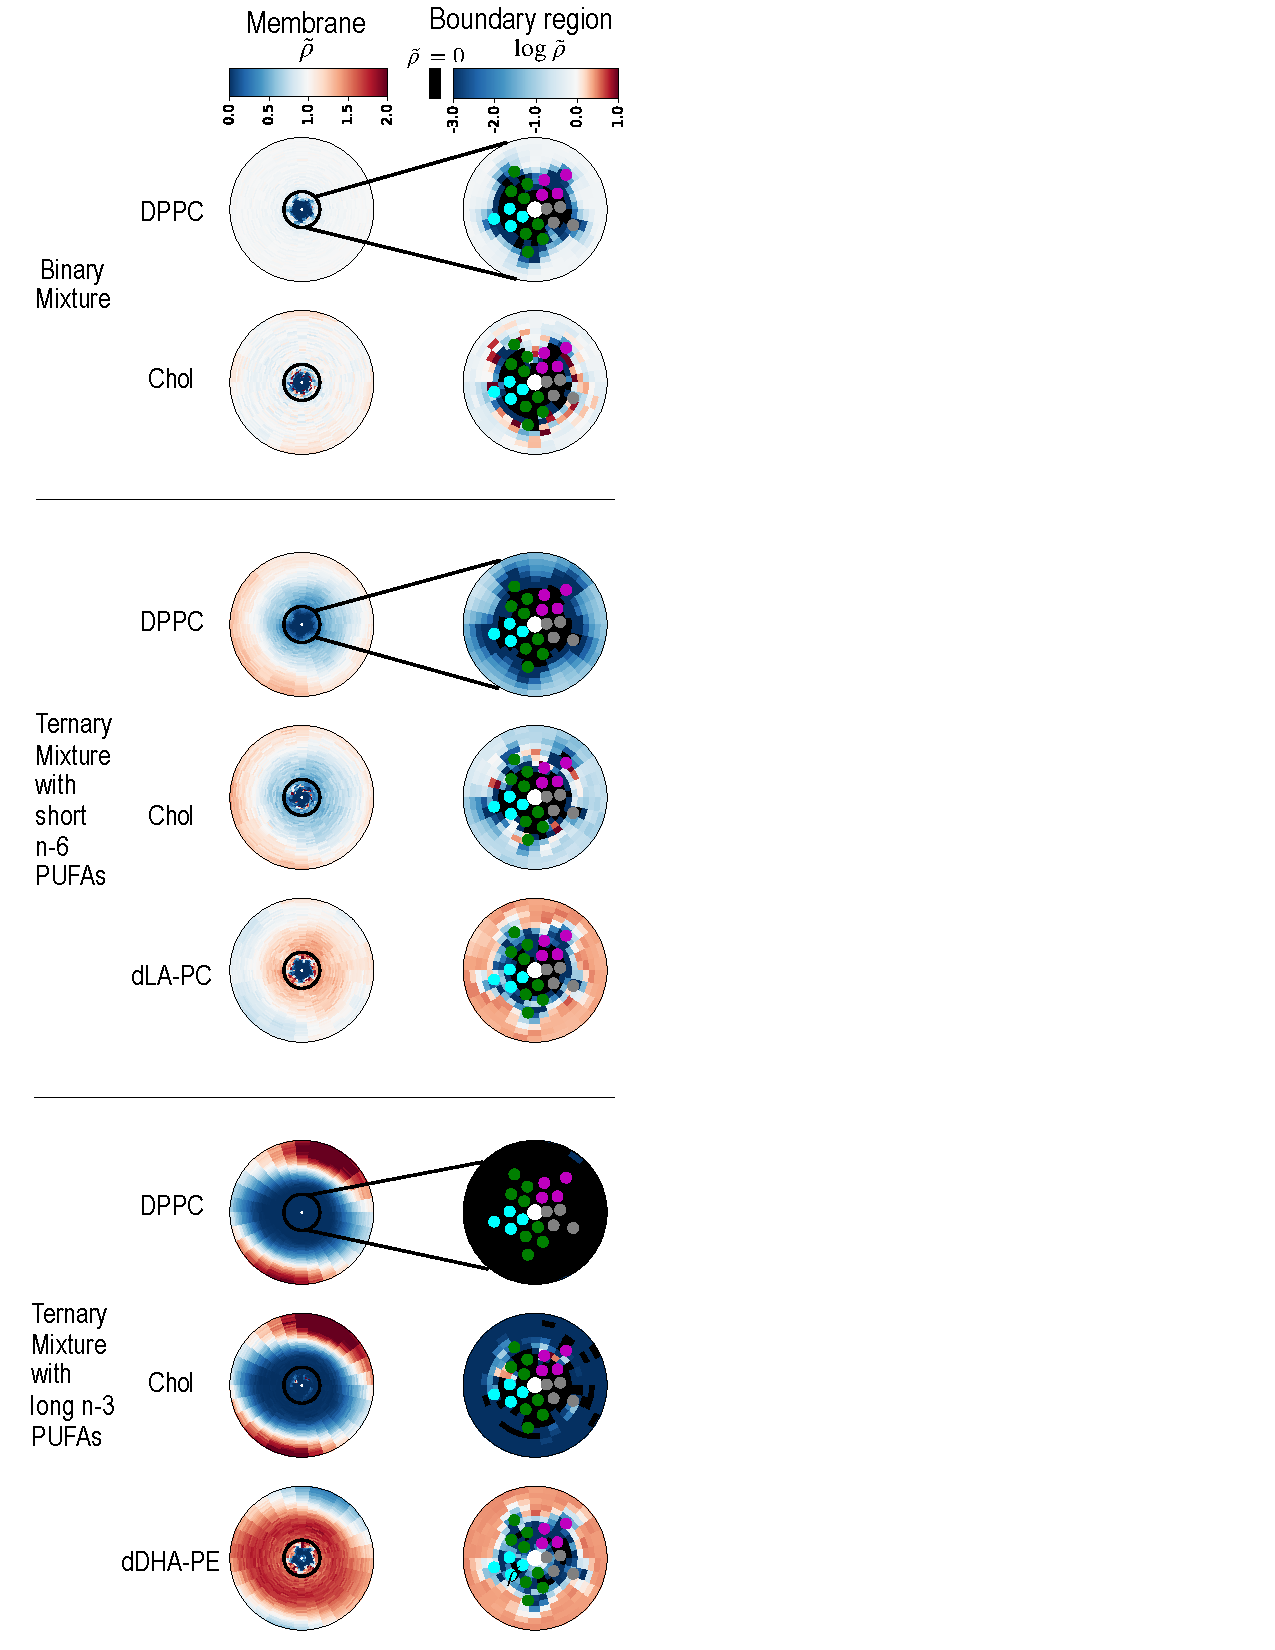
\includegraphics[width=1\linewidth]{ComparativeHeatMap.pdf}
		\caption{\liam{(left) Lipid distribution at long length scales. (right) Lipid bead distribution local to the nAChR TMD helices.} (Left) Heat maps representing normalized average lipid density are calculated over the last half of a $10 \mu$s simulation with composition DPPC:PUFA:CHOL 2:2:1 (as in Figure \ref{fig:fig1}A and B)  or  DPPC:CHOL 4:1 (as in Figure \ref{fig:binary} A and C) . ${\tilde{\rho}}_{a}$ is normalized by expected density based on composition (defined in eq \ref{eq:Rt}); white indicates no enrichment or depletion. \liam{The circle at the center of each heat map represents the right side figures. These heat maps to not include the \nachr~subunits plotted.}  (Right) Data is identical to the left figure but colorscale is adjusted and logarithmic density is shown, for representation of specific lipid binding. All beads for each lipid were used to calculate the density distribution, and density was normalized by expectation based on composition and number of beads per molecule.  Bins in which no density for the given lipid type was detected are shown as black.  Circles represent nAChR TMD helices, colored by subunit as in Fig. \ref{fig:binary} A.\grace{Update caption once figure is finalized}}
		\label{fig:sorting}
	\end{figure*}

	%\begin{figure}[h!]
%		\center
%		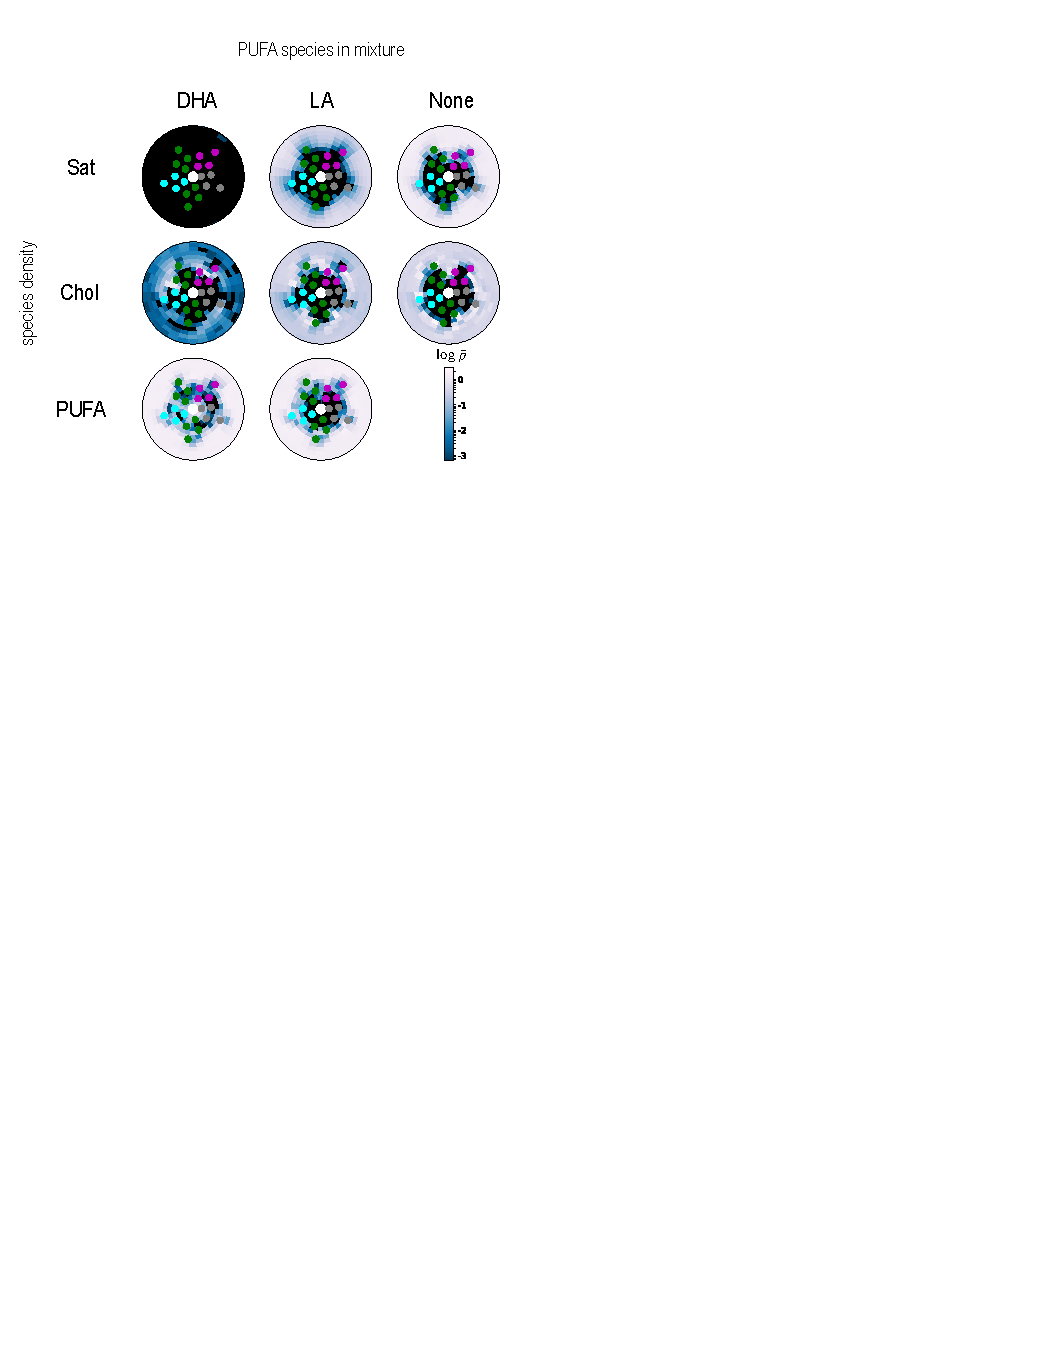
\includegraphics[width=1\linewidth]{Fig3.pdf}%
%		\caption{Lipid bead distribution local to the nAChR TMD helices. Data is identical to Fig. \ref{fig:sorting} but colorscale is adjusted and logarithmic density is shown, for representation of specific lipid binding. All beads for each lipid were used to calculate the density distribution, and density was normalized by expectation based on composition and number of beads per molecule.  Bins in which no density for the given lipid type was detected are shown as black.  Circles represent nAChR TMD helices, colored by subunit as in Fig. \ref{fig:binary} A. } 
%		\label{fig:fig3}
%	\end{figure}
	%Heat maps in Figure \ref{fig:fig3} \textbf{b} show the average density of cholesterol $(\rho_{Chol})$ within a membrane. $\rho$ is generally defined by equation \ref{eq:R}. In \ref{fig:fig3}b left, the system has a composition DHA-PE:DPPC:Chol 40:40:20. Chol is found in the $l_o$ domain. However, while $\beta$ subunit is partitioned into the $l_d$ phase, there is significant increase in $\rho_{Chol}$ within the $\beta$ subunit. In \ref{fig:fig3} \textbf{b right} DLiPC:DPPC:Chol 40:40:20, $\rho_{Chol}$ is greatest throughout the protein, with largest value within $\delta$ subunit.

	%Figure \ref{fig:fig3} shows the average of three replicas of PUFA:DPPC:Chol 40:40:20, where the PUFA is either DHA-PE or DLiPC. Protein chain locations are also averaged, resulting in a compressed area. Cholesterol is still observed to partition near or within nAChR and in the $l_o$ phase in systems containing DHA. It is highly dispersed within the bulk membrane and embedded with nAChR in systems with DLiPC. Saturated lipids in both series of systems tend to form the bulk membrane, and do not readily interact with nAChR. PUFAs tend form a dense boundary area around nAChR. Chol is observed to embed within or between subunits indiscriminately.

	\begin{figure}[h!]
		\center
		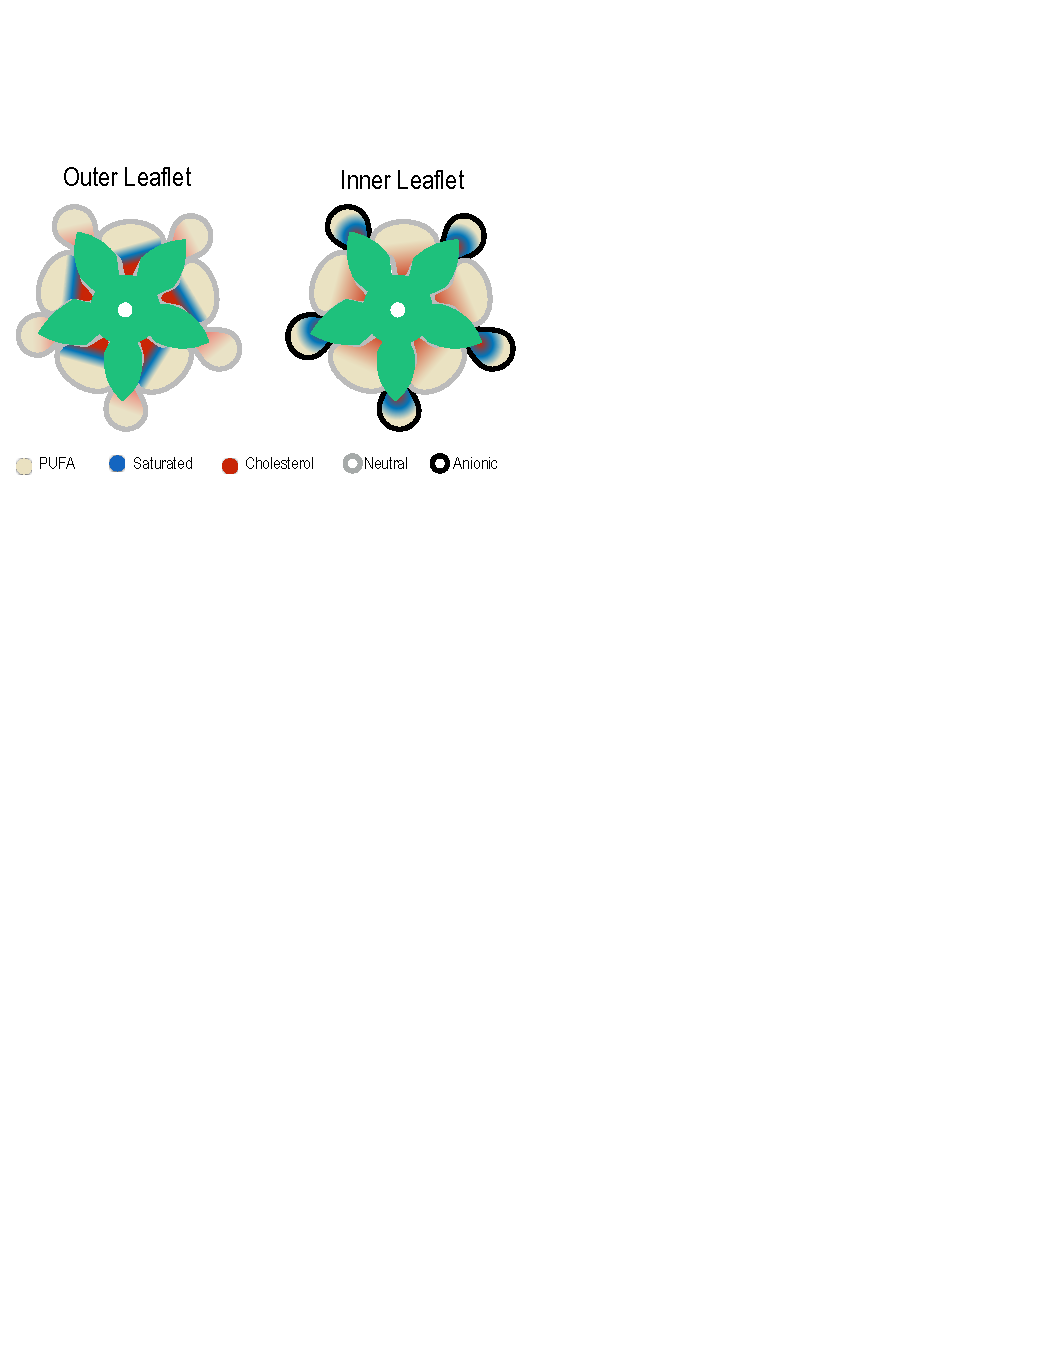
\includegraphics[width=1\linewidth]{Summary.pdf}
		\caption{ Embedded lipids in the nAChR. Main image: Representative frame from equilibrated small membrane simulation of nAChR in 2:2:1 DPPC:DHA-PE:CHOL. Backbone beads of the TMD helices are colored by subunit as in Figure \ref{fig:fig2}; side-chain beads are not shown.  Both DHA-PE (white) and cholesterol (red) equilibrate to embedded sites in the subunit center and subunit interfaces, although most cholesterol is found in the $\lo$ phase with DPPC (blue). Inset : Cryo-EM density of nAChR from \cite{Miyazawa2003} as rendered in \cite{Brannigan_Embedded_2008}; dark blue indicates high density, white is medium density, and red is low density. } 
		\label{fig:sum}
	\end{figure}

	 
